\chapter{Proposed Methodology}
\label{chp3}
In the previous chapter, we have discussed the theories that support this project related to
the School Management System. In this chapter we will proposed our methodology for this
project while giving details about proposed methodology ER diagram, database implementation, software being used in this project.
\section{Proposed Methodology}
The proposed School Management System (SMS) will dealt with all this issues that the current system is facing all the process
are suggested to be executed more efficiently and effectively without any difficulties.\\
All the processes and operations in the current school management system are executed
manually inform of paper. This makes all the process difficult to the school administrators,
teachers and other officials to carry out. All the records of students, staffs and many other
important data related to the school are kept indifferent files. There is a need to rehabilitate their system to
computerized school management system so that that they will efficiently carry their work
without any difficulties.\\\\ 
The proposed system will remove the all the manual process of
,updating record, searching data eliminate registering student and teachers, forming classes
,assigning teachers , entering student exam details, generating time table, uploading student
result, and many other functionalities needed by the end users. By automating the system, it will
extremely improve the way school function, which will also improve efficiency and
managerial effectiveness\cite{burke2003practice}.\\\\
There is also high risk of losing data in the current manual system
because school management use to store all their data in the same place but different files.This problem will be address by introducing
new feature in to the proposed SMS that will enable the administrator
to store information about, students, teachers, subject, exam details, and time table, attendance
and so on, and also the teacher will be able to enter student�s marks and so that back up can be
done when any data lost etc. All this features will be simplified in an easiest way so that they will
carry out their workloads efficiently without any difficulties.
\section{Entity Relation Diagram}
\begin{figure}[H]  %h=positioning
\begin{center}
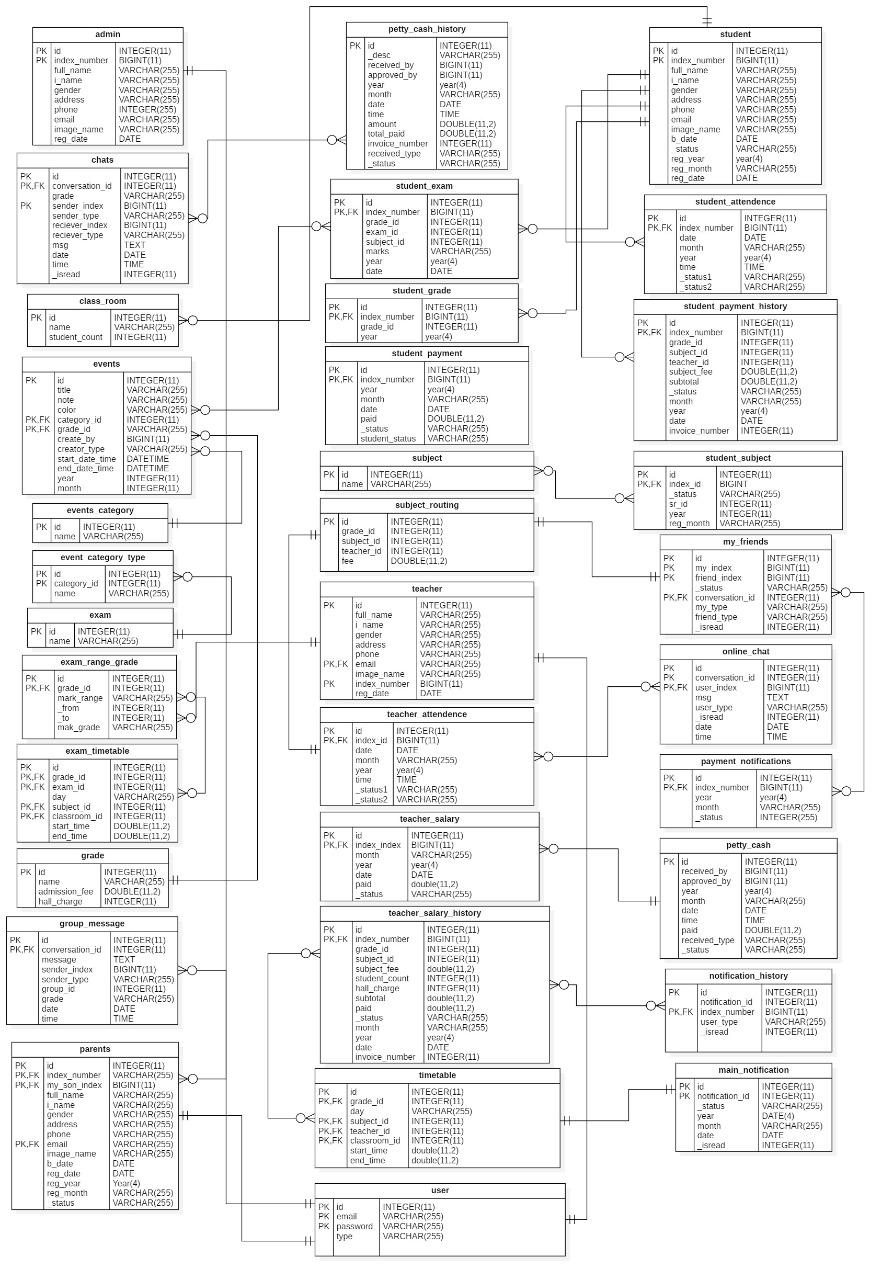
\includegraphics[scale=0.50]{Chapter3/ERdiagram}
\caption{Entity Relation Diagram of SMS}
\label{BMRDevice}
\end{center}
\end{figure}
\section{Tools/Platform, and Softwares}
Following are the software and their requirements which we have used for this project.
\subsection{MySQL Workbench CE 8.0}
MySQL Workbench is a visual database design tool that integrates SQL development, administration, database design, creation and maintenance into a single integrated development environment for the MySQL database system. It is the successor to DBDesigner 4 from fabFORCE.net, and replaces the previous package of software, MySQL GUI Tools Bundle.
\begin{figure}[H]  %h=positioning
\begin{center}
\includegraphics[scale=0.2]{Chapter3/mySQL}
\caption{MySQL Logo}
\label{mySQL}
\end{center}
\end{figure}
\subsection{HTML}
The HyperText Markup Language, or HTML is the standard markup language for documents designed to be displayed in a web browser. It can be assisted by technologies such as Cascading Style Sheets (CSS) and scripting languages such as JavaScript.
 \begin{figure}[H]  %h=positioning
\begin{center}

\includegraphics[scale=0.2]{Chapter3/html}
\caption{HTML Logo}
\label{html}
\end{center}
\end{figure}
\subsection{PHP}
PHP is a general-purpose scripting language geared towards web development. It was originally created by Danish-Canadian programmer Rasmus Lerdorf in 1994. The PHP reference implementation is now produced by The PHP Group. PHP originally stood for Personal Home Page, but it now stands for the recursive initialism PHP: Hypertext Preprocessor. 
\begin{figure}[H]  %h=positioning
\begin{center}

\includegraphics[scale=0.2]{Chapter3/php}
\caption{PHP Logo}
\label{php}
\end{center}
\end{figure}
\subsection{XAMPP}
XAMPP (/'z�mp/ or /'?ks.�mp/) is a free and open-source cross-platform web server solution stack package developed by Apache Friends, consisting mainly of the Apache HTTP Server, MariaDB database, and interpreters for scripts written in the PHP and Perl programming languages. Since most actual web server deployments use the same components as XAMPP, it makes transitioning from a local test server to a live server possible. 
\begin{figure}[H]  %h=positioning
\begin{center}

\includegraphics[scale=0.2]{Chapter3/xampp}
\caption{XAMPP Logo}
\label{xampp}
\end{center}
\end{figure}
\section{Project Working Manual}
Following steps will provide a complete guide to run your project using XAMPP.
\begin{enumerate}
\item Download �XAMPP� and install that. \url{https://www.apachefriends.org/download.html}
\item Search �XAMPP Control Panel� in the search bar and open that.
\begin{figure}[H]  %h=positioning
\begin{center}
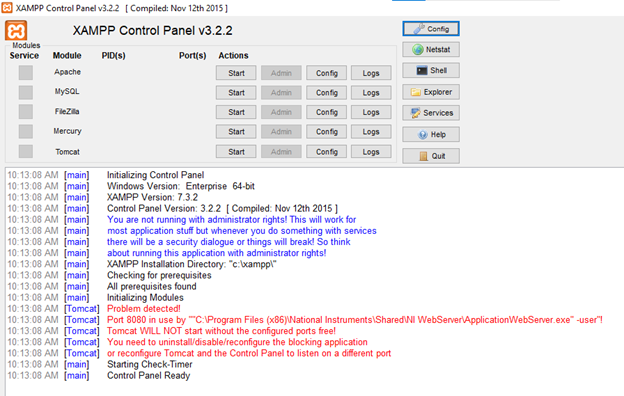
\includegraphics[scale=1]{Chapter3/step2}
\caption{XAMPP Control Panel View}
\label{xampp}
\end{center}
\end{figure}
\item Start �Apache� and �MySQL�.
\begin{figure}[H]  %h=positioning
\begin{center}
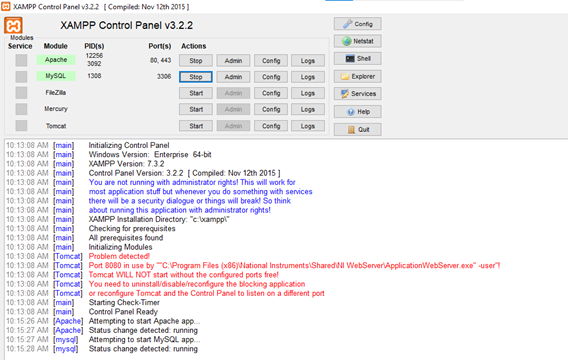
\includegraphics[scale=1]{Chapter3/step3}
\caption{XAMPP Control Panel View}
\label{xampp}
\end{center}
\end{figure}
\item If MySQL doesn't�t start, Search �services� on search bar.
\begin{figure}[H]  %h=positioning
\begin{center}
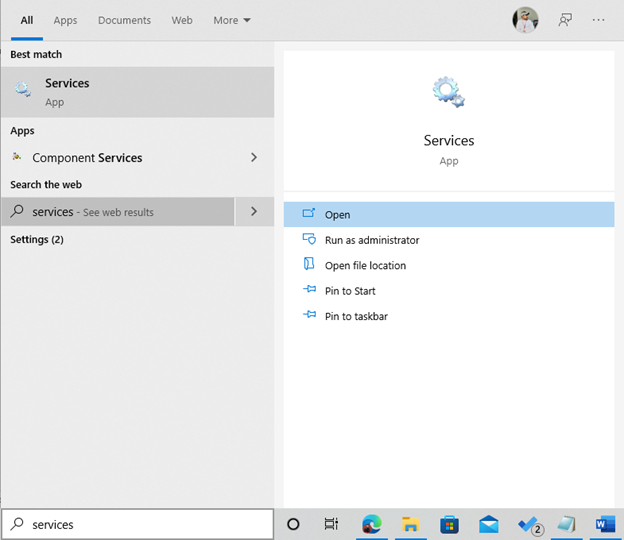
\includegraphics[scale=0.75]{Chapter3/step4}
\caption{Search Panel View}
\label{xampp}
\end{center}
\end{figure}
\item Search �mySQL�, right click on that and stop from there.
\begin{figure}[H]  %h=positioning
\begin{center}
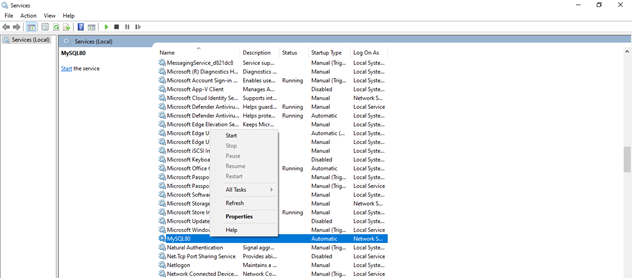
\includegraphics[scale=1]{Chapter3/step5}
\caption{Services Panel View}
\label{xampp}
\end{center}
\end{figure}
\item Go back to �XAMPP Control Panel� and Start �Apache� and �MySQL�.
\begin{figure}[H]  %h=positioning
\begin{center}
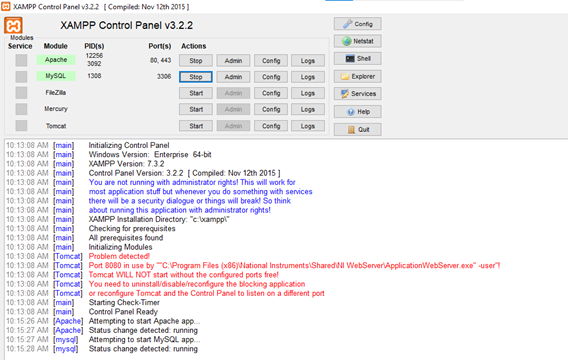
\includegraphics[scale=1]{Chapter3/step3}
\caption{XAMPP Control Panel View}
\label{xampp}
\end{center}
\end{figure}
\item Find the project folder and copy from there.
\begin{figure}[H]  %h=positioning
\begin{center}
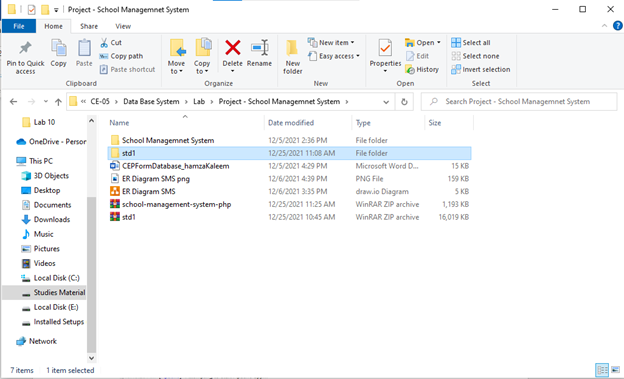
\includegraphics[scale=1]{Chapter3/step6}
\caption{File Location to be Copied}
\label{xampp}
\end{center}
\end{figure}
\item Go to �xampp� folder where you installed this, than go to htdocs and paste the project file there.
\begin{figure}[H]  %h=positioning
\begin{center}
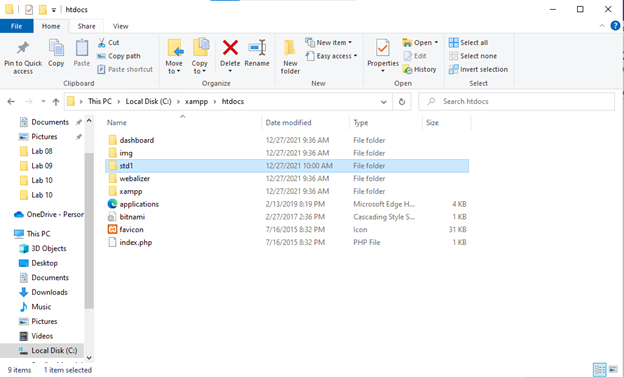
\includegraphics[scale=1]{Chapter3/step7}
\caption{Destination File Location}
\label{xampp}
\end{center}
\end{figure}
\item Open any browser and search \url{http://localhost/phpmyadmin/}
\begin{figure}[H]  %h=positioning
\begin{center}
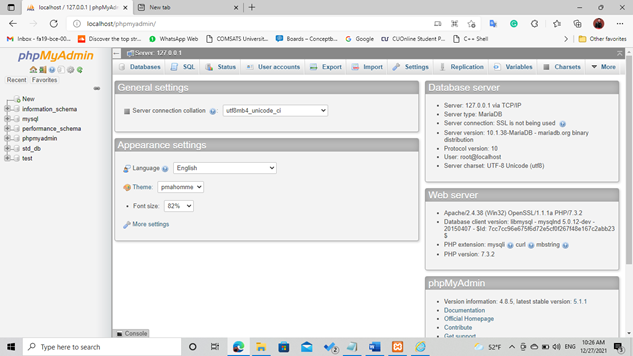
\includegraphics[scale=1]{Chapter3/step8}
\caption{phpmyadmin view}
\label{xampp}
\end{center}
\end{figure}
\item Click on the databases
\begin{figure}[H]  %h=positioning
\begin{center}
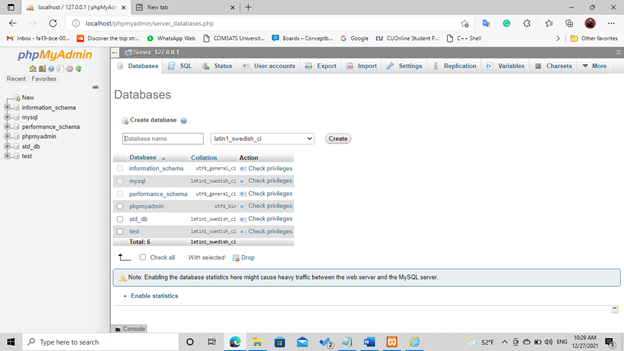
\includegraphics[scale=1]{Chapter3/step9}
\caption{phpmyadmin Database view}
\label{xampp}
\end{center}
\end{figure}
\item Enter the name of the database of the project and press create e.g., std\_db
\begin{figure}[H]  %h=positioning
\begin{center}
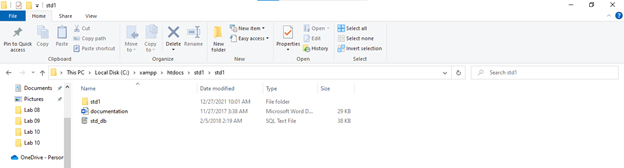
\includegraphics[scale=1]{Chapter3/step10}
\caption{phpmyadmin view}
\label{xampp}
\end{center}
\end{figure}
\begin{figure}[H]  %h=positioning
\begin{center}
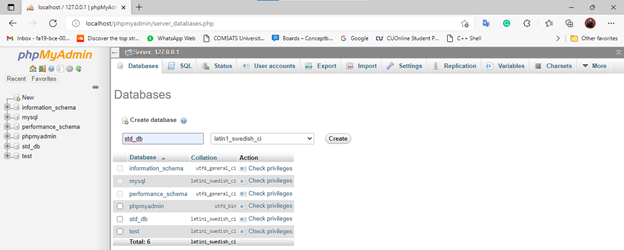
\includegraphics[scale=0.75]{Chapter3/step11}
\caption{phpmyadmin view}
\label{xampp}
\end{center}
\end{figure}
\begin{figure}[H]  %h=positioning
\begin{center}
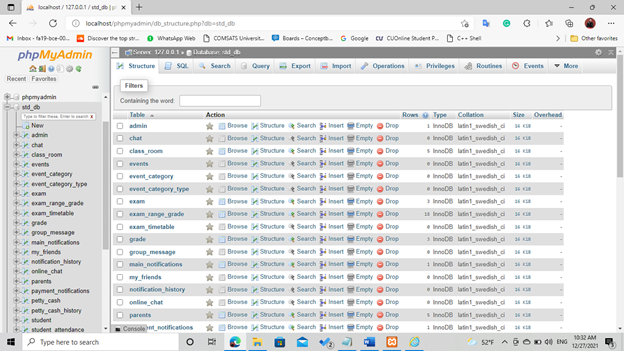
\includegraphics[scale=1]{Chapter3/step12}
\caption{phpmyadmin view}
\label{xampp}
\end{center}
\end{figure}
\item Click on the import
\begin{figure}[H]  %h=positioning
\begin{center}
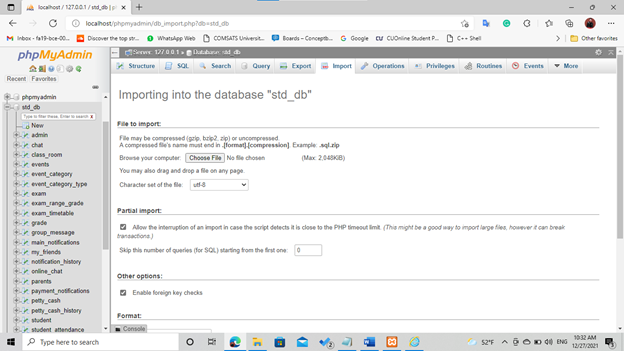
\includegraphics[scale=1]{Chapter3/step13}
\caption{phpmyadmin view}
\label{xampp}
\end{center}
\end{figure}
\item Choose the same database file and import this
\begin{figure}[H]  %h=positioning
\begin{center}
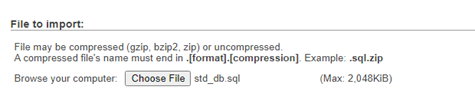
\includegraphics[scale=1]{Chapter3/step14}
\caption{phpmyadmin view}
\label{xampp}
\end{center}
\end{figure}
\item Scroll down and press on the �go�
\begin{figure}[H]  %h=positioning
\begin{center}
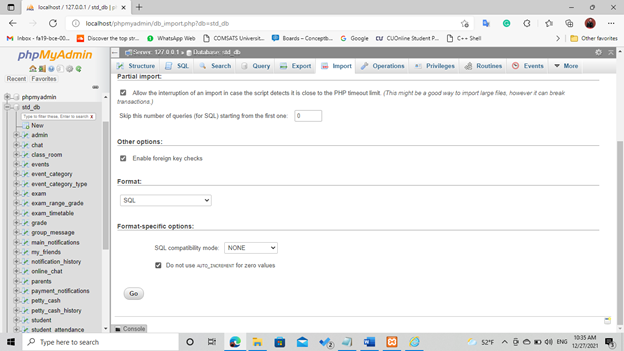
\includegraphics[scale=1]{Chapter3/step15}
\caption{phpmyadmin view}
\label{xampp}
\end{center}
\end{figure}
\item Open a new tab and search �localhost/projectFoldername� e.g., localhost/std1
\begin{figure}[H]  %h=positioning
\begin{center}
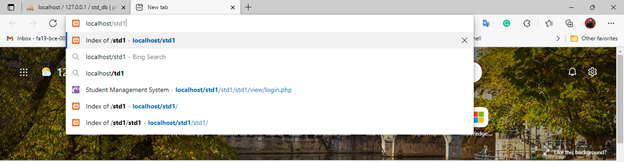
\includegraphics[scale=1]{Chapter3/step16}
\caption{localhost/std1 view}
\label{xampp}
\end{center}
\end{figure}
\item Click on the project name again.
\begin{figure}[H]  %h=positioning
\begin{center}
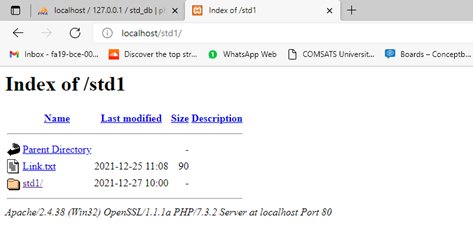
\includegraphics[scale=1]{Chapter3/step17}
\caption{localhost/std1 view}
\label{xampp}
\end{center}
\end{figure}
\item Here you go�
\begin{figure}[H]  %h=positioning
\begin{center}
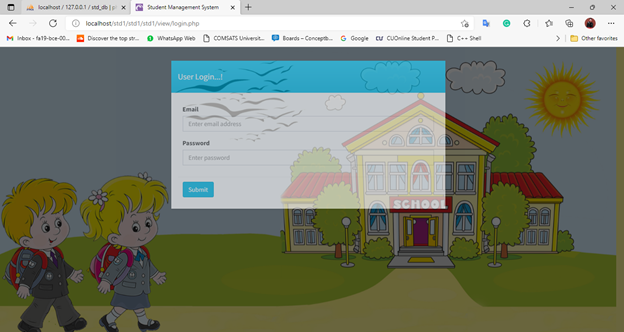
\includegraphics[scale=1]{Chapter3/step18}
\caption{Project Front Page}
\label{xampp}
\end{center}
\end{figure}
\end{enumerate}